\chap{八}{薛寶釵小恙梨香院 賈寶玉大醉絳芸軒}

\begin{parag}
    \begin{note}蒙:幻情濃處故多嗔,豈獨顰兒愛妒人。莫把心思勞展轉,百年事業總非真。\end{note}
\end{parag}


\begin{parag}
    題曰:
\end{parag}


\begin{poem}
    \begin{pl}古鼎新烹鳳髓香,那堪翠斝貯瓊漿。\end{pl}

    \begin{pl}莫道綺縠無風韻,試看金娃對玉郎。\end{pl}
\end{poem}


\begin{parag}
    話說鳳姐和寶玉回家,見過衆人。寶玉先便回明賈母秦鍾要上家塾之事,自己也有了個伴讀的朋友,正好發奮,\begin{note}甲側:未必。\end{note}又著實的稱讚秦鐘的人品行事,最使人憐愛。鳳姐又在一旁幫著說“過日他還來拜老祖宗”等語,說的賈母喜歡起來。\begin{note}甲側:止此便十成了,不必繁文再表,故妙。偷渡金針法。\end{note}鳳姐又趁勢請賈母后日過去看戲。賈母雖年老,卻極有興頭。\begin{note}甲側:爲賈母寫傳。\end{note}至後日,又有尤氏來請,遂攜了王夫人、林黛玉,寶玉等過去看戲。至晌午,賈母便回來歇息了。\begin{note}甲雙夾:敘事有法,若只管寫看戲,便是一無見世面之暴發貧婆矣。寫“隨便”二字,興高則往,興敗則回,方是世代封君正傳。且“高興”二字,又可生出多少文章來。\end{note}王夫人本是好清淨的,\begin{note}甲雙夾:偏與邢夫人相犯,然卻是各有各傳。\end{note}見賈母回來也就回來了。然後鳳姐坐了首席,盡歡至晚無話。\begin{note}甲側:細甚,交代畢。\end{note}
\end{parag}


\begin{parag}
    卻說寶玉因送賈母回來,待賈母歇了中覺,意欲還去看戲取樂,又恐擾的秦氏等人不便,\begin{note}甲側:全是體貼功夫。\end{note}因想起近日薛寶釵在家養病,未去親候,意欲去望他一望。若從上房后角門過去,又恐遇見別事纏繞,再或可巧遇見他父親,\begin{note}甲側:本意正傳,實是曩時苦惱,嘆嘆!\end{note}更爲不妥,\begin{note}甲側:細甚。\end{note}寧可繞遠路罷了。當下衆嬤嬤丫鬟伺候他換衣服,見他不換,仍出二門去了。衆嬤嬤丫鬟只得跟隨出來,還只當他去那府中看戲。誰知到穿堂,便向東向北繞廳後而去。偏頂頭遇見了門下清客相公詹光、\begin{note}甲側:妙!蓋沾光之意。\end{note}單聘仁\begin{note}甲側:更妙!蓋善於騙人之意。\end{note}二人走來,一見了寶玉,便都笑著趕上來,一個抱住腰,一個攜著手,都道:“我的菩薩哥兒,\begin{note}甲側:沒理沒倫,口氣畢肖。\end{note}我說作了好夢呢,好容易得遇見了你。”說著,請了安,又問好,勞叨了半日,方纔走開。\begin{note}甲眉:一路用淡三色烘染、行雲流水之法,寫出貴公子家常不即不離氣致。經歷過者則喜其寫真,未經者恐不免嫌繁。\end{note}老嬤嬤叫住,因問:“你二位爺是從老爺跟前來的不是?”\begin{note}甲側:爲玉兄一人,卻人人俱有心事,細緻。\end{note}二人點頭\begin{note}甲側:使人起遐思。\end{note}道:“老爺在夢坡齋\begin{note}甲側:妙!夢遇坡仙之處也。\end{note}小書房裏歇中覺呢,不妨事的。”\begin{note}甲側:玉兄知己。一笑。\end{note}一面說,一面走了。說的寶玉也笑了。於是轉彎向北奔梨香院來。可巧銀庫房的總領名喚吳新登\begin{note}甲側:妙!蓋雲無星戥也。\end{note}與倉上的頭目名戴良,\begin{note}甲側:妙!蓋雲大量也。\end{note}還有幾個管事的頭目,共有七個人,從帳房裏出來,一見了寶玉,趕來都一齊垂手站住。獨有一個買辦名喚錢華,\begin{note}甲雙夾:亦錢開花之意。隨事生情,因情得文。\end{note}因他多日未見寶玉,忙上來打千兒請安,寶玉忙含笑攜他起來。衆人都笑說:“前兒在一處看見二爺寫的斗方兒,字法越發好了,多早晚兒賞我們幾張貼貼。”\begin{note}甲眉:餘亦受過此騙,今閱至此,赧然一笑。此時有三十年前向餘作此語之人在側,觀其形已皓首駝腰矣,乃使彼亦細聽此數語,彼則潸然泣下,餘亦爲之敗興。\end{note}寶玉笑道:“在那裏看見了?”衆人道:“好幾處都有,都稱讚的了不得,還和我們尋呢。”寶玉笑道:“不值什麼,你們說與我的小幺兒們就是了。”一面說,一面前走,衆人待他過去,方都各自散了。\begin{note}甲雙夾:未入梨香院,先故作若許波瀾曲折。瞧他無意中又寫出寶玉寫字來,固是愚弄公子閒文,然亦是暗逗寶玉曆來文課事。不然,後文豈不太突?\end{note}
\end{parag}


\begin{parag}
    閒言少述,\begin{note}甲雙夾:此處用此句最當。\end{note}且說寶玉來至梨香院中,先入薛姨媽室中來,正見薛姨媽打點針黹與丫鬟們呢。寶玉忙請了安,薛姨媽忙一把拉了他,抱入懷內,笑說:“這們冷天,我的兒,難爲你想著來,快上炕來坐著罷。”命人倒滾滾的茶來。寶玉因問:“哥哥不在家?”薛姨媽嘆道:“他是沒籠頭的馬,天天逛不了,那裏肯在家一日。”寶玉道:“姐姐可大安了?”薛姨媽道:“可是呢,你前兒又想著打發人來瞧他。他在裏間不是,你去瞧他,裏間比這裏暖和,那裏坐著,我收拾收拾就進去和你說話兒。”寶玉聽說,忙下了炕來至裏間門前,只見吊著半舊的紅紬軟簾。\begin{note}甲側:從門外看起,有層次。\end{note}寶玉掀簾一邁步進去,先就看見薛寶釵坐在炕上作針線,頭上挽著漆黑油光的纂兒,蜜合色棉襖,玫瑰紫二色金銀鼠比肩褂,蔥黃綾棉裙,一色半新不舊,看去不覺奢華。脣不點而紅,眉不畫而翠,臉若銀盆,眼如水杏。罕言寡語,人謂藏愚,安分隨時,自雲守拙。\begin{note}甲雙夾:這方是寶卿正傳。與前寫黛玉之傳一齊參看,各極其妙,各不相犯,使其人難其左右於毫末。甲眉:畫神鬼易,畫人物難。寫寶卿正是寫人之筆,若與黛玉並寫更難。今作者寫得一毫難處不見,且得二人真體實傳,非神助而何?\end{note}寶玉一面看,一面問:“姐姐可大愈了?”寶釵抬頭\begin{note}甲側:與寶玉邁步針對。\end{note}只見寶玉進來,\begin{note}甲雙夾:此則神情盡在煙飛水逝之間,一展眼便失於千里矣。\end{note}連忙起身含笑答說:“已經大好了,倒多謝記掛著。”說著,讓他在炕沿上坐了,即命鶯兒斟茶來。一面又問老太太、姨媽安,別的姊妹們都好。\begin{note}甲側:這是口中如此。\end{note}一面\begin{note}甲側:“一面”二,口中眼中,神情俱到。\end{note}看寶玉頭上戴著縲絲嵌寶紫金冠,額上勒著二龍搶珠金抹額,身上穿著秋香色立白狐腋箭袖,腰繫五色蝴蝶鸞絛,項上掛著長命鎖、記名符,另外有一塊落草時銜下來的寶玉。寶釵因笑說道:“成日家說你的這玉,究竟未曾細細的賞鑑,我今兒倒要瞧瞧。”\begin{note}甲雙夾:自首回至此,回回說有通靈玉一物,餘亦未曾細細賞鑑,今亦欲一見。\end{note}說著便挪近前來。寶玉亦湊了上去,從項上摘了下來,遞在寶釵手內。寶釵託於掌上,\begin{note}甲雙夾:試問石兄:此一託,比在青埂峯下猿啼虎嘯之聲何如?甲眉:餘代答曰:“遂心如意。”\end{note}只見大如雀卵,\begin{note}甲側:體。\end{note}燦若明霞,\begin{note}甲側:色。\end{note}瑩潤如酥,\begin{note}甲側:質。\end{note}五色花紋纏護。\begin{note}甲側:文。\end{note}這就是大荒山中青埂峯下的那塊頑石的幻相。\begin{note}甲側:註明。\end{note}後人曾有詩嘲雲:
\end{parag}


\begin{poem}
    \begin{pl}女媧煉石已荒唐,又向荒唐演大荒。\end{pl}

    \begin{pl}失去幽靈真境界,幻來親就假皮囊。\end{pl}
    \begin{note}甲側:二語可入道,故前引莊叟祕訣。\end{note}

    \begin{pl}好知運敗金無彩,堪嘆時乖玉不光。\end{pl}
    \begin{note}甲側:又夾入寶釵,不是虛圖對得工。二語雖粗,本是真情,然此等詩只宜如此,爲天下兒女一哭。\end{note}

    \begin{pl}白骨如山忘姓氏,無非公子與紅妝!\end{pl}
    \begin{note}甲側:批得好。末二句似與題不切,然正是極貼切語。\end{note}
\end{poem}


\begin{parag}
    那頑石亦曾記下他這幻相併癩僧所鐫的篆文,今亦按圖畫於後。但其真體最小,方能從胎中小兒口內銜下。今若按其體畫,恐字跡過於微細,使觀者大廢眼光,亦非暢事。故今只按其形式,無非略展些規矩,使觀者便於燈下醉中可閱。今註明此故,方無“胎中之兒口有多大,怎得銜此狼犺蠢大之物等語之謗。\begin{note}甲眉:又忽作此數語,以幻弄成真,以真弄成幻。真真假假,恣意遊戲於筆墨之中,可謂狡猾之至。作人要老誠,作文要狡猾。\end{note}
\end{parag}

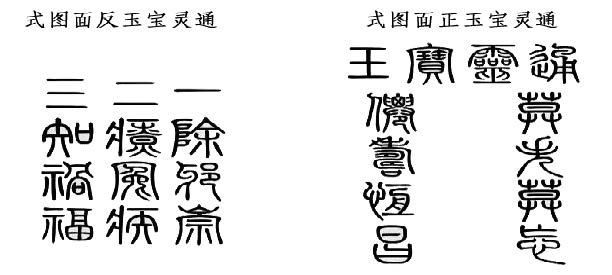
\includegraphics{1-80/8-1}

\begin{qute}

    \begin{parag}\textbf{通靈寶玉反面圖式} \newline
        \indent 三二一\newline
        \indent 知療除\newline
        \indent 禍冤邪\newline
        \indent 福疾崇\newline
    \end{parag}


    \begin{parag}
        \textbf{通靈寶玉正面圖式}\newline
        \indent 仙莫\newline
        \indent 壽失\newline
        \indent 恆莫\newline
        \indent 昌忘\newline
    \end{parag}
\end{qute}


\begin{parag}
    寶釵看畢,\begin{note}甲雙夾:餘亦想見其物矣。前回中總用草蛇灰線寫法,至此方細細寫出,正是大關節處。\end{note}又從新翻過正面來細看,\begin{note}甲側:可謂真奇之至。\end{note}口內念道:“莫失莫忘,仙壽恆昌。”\begin{note}甲側:是心中沉吟,神理。甲眉:《石頭記》立誓一筆不寫一家文字。\end{note}唸了兩遍,乃回頭向鶯兒笑道:“你不去倒茶,也在這裏發呆作什麼?”\begin{note}甲雙夾:請諸公掩卷合目想其神理,想其坐立之勢,想寶釵面上口中。真妙!\end{note}鶯兒嘻嘻笑道:“我聽這兩句話,倒象和姑娘的項圈上的兩句話是一對兒。”\begin{note}甲雙夾:又引出一個金項圈來,鶯兒口中說出方妙。甲眉:恨顰兒不早來聽此數語,若使彼聞之,不知又有何等妙論趣語以悅我等心臆。\end{note}寶玉聽了,忙笑道:“原來姐姐那項圈上也有八個字,\begin{note}甲雙夾:補出素日眼中雖見而實未留心。\end{note}我也鑑賞鑑賞!”寶釵道:“你別聽他的話,沒有什麼字。”寶玉笑央:“好姐姐,你怎麼瞧我的了呢。”寶釵被纏不過,因說道:“也是個人給了兩句吉利話兒,所以鏨上了,叫天天帶著,不然,沉甸甸的有什麼趣兒。”\begin{note}甲雙夾:一句罵死天下濃妝豔飾富貴中之脂妖粉怪。\end{note}一面說,一面解了排扣,\begin{note}甲側:細。\end{note}從裏面大紅襖上將那珠寶晶瑩黃金燦爛的瓔珞掏將出來。\begin{note}甲雙夾:按,瓔珞者,頸飾也!想近俗即呼爲項圈者是矣。\end{note}寶玉忙託了鎖看時,果然一面有四個篆字,兩面八字,共成兩句吉讖。亦曾按式畫下形相:
\end{parag}

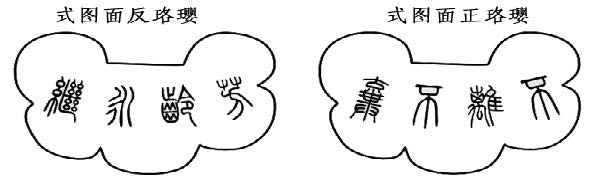
\includegraphics[]{1-80/8-2}

\begin{qute}

    \begin{parag}
        \textbf{瓔珞反面式}
    \end{parag}


    \begin{parag}
        音注云:芳齡永繼。\begin{note}甲側:合前讀之,豈非一對?\end{note}
    \end{parag}


    \begin{parag}
        \textbf{瓔珞正面式}
    \end{parag}


    \begin{parag}
        音注云:不離不棄。
    \end{parag}
\end{qute}


\begin{parag}
    寶玉看了,也念了兩遍,又念自己的兩遍,因笑問:“姐姐這八個字倒真與我的是一對。”\begin{note}甲雙夾:餘亦謂是一對,不知干支中四注八字可與卿亦對否?甲眉:花看半開,酒飲微醉,此文字是也。\end{note}鶯兒笑道:“是個癩頭和尚送的,他說必須鏨在金器上……“\begin{note}和尚在幻境中作如此勾當,亦屬多事。\end{note}寶釵不待說完,便嗔他不去倒茶,\begin{note}甲側:寫寶釵身份。蒙側:雲龍顯影法,好看煞!\end{note}一面又問寶玉從那裏來。\begin{note}甲側:妙神妙理,請觀者自思。\end{note}
\end{parag}


\begin{parag}
    寶玉此時與寶釵就近,只聞一陣陣涼森森甜絲絲的幽香,\begin{note}蒙側:這方是花香襲人正意。\end{note}竟不知系何香氣,遂問:“姐姐燻的是什麼香?我竟從未聞見過這味兒。”\begin{note}甲側:不知比“羣芳髓”又何如?\end{note}寶釵笑道:“我最怕薰香,好好的衣服,燻的煙燎火氣的。”\begin{note}甲側:真真罵死一干濃妝豔飾鬼怪。\end{note}寶玉道:“既如此,這是什麼香?”寶釵想了一想,笑道:“是了,是我早起吃了丸藥的香氣。”\begin{note}甲側:點“冷香丸”。\end{note}寶玉笑道:“什麼丸藥這麼好聞?好姐姐,給我一丸嚐嚐。”\begin{note}甲雙夾:仍是小兒語氣。究竟不知別個小兒,只寶玉如此。\end{note}寶釵笑道:“又混鬧了,一個藥也是混喫的?”
\end{parag}


\begin{parag}
    一語未了,忽聽外面人說:“林姑娘來了。”\begin{note}甲側:緊處愈緊,密不容針之文。\end{note}話猶未了,林黛玉已搖搖\begin{note}甲側:二字畫出身份。\end{note}的走了進來,一見了寶玉,便笑道:“噯喲,我來的不巧了!”\begin{note}甲側:奇文,我實不知顰兒心中是何丘壑。\end{note}寶玉等忙起身笑讓坐,寶釵因笑道:“這話怎麼說?”黛玉笑道:“早知他來,我就不來了。”寶釵道:“我更不解這意。”黛玉笑道:“要來一羣都來,要不來一個也不來,今兒他來了,明兒我再來,如此間錯開了來著,豈不天天有人來了?\begin{note}甲側:強詞奪理。\end{note}也不至於太冷落,也不至於太熱鬧了。\begin{note}甲側:好點綴。\end{note}姐姐如何反不解這意思?”\begin{note}甲雙夾:吾不知顰兒以何物爲心爲齒爲口爲舌,實不知胸中有何丘壑。\end{note}
\end{parag}


\begin{parag}
    寶玉因見他外面罩著大紅羽緞對衿褂子,\begin{note}甲側:岔開文字,避繁章法,妙極妙極!\end{note}\begin{note}蒙側:又一轉換。若無此則必有寶玉之窮究,寶釵之重複,加長無味。此等文章是《西遊記》的請觀世音菩薩,菩薩一到,無不掃地完結者。\end{note}因問:“下雪了麼?”地下婆娘們道:“下了這半日雪珠兒了。”寶玉道:“取了我的斗篷來不曾?”黛玉便道:“是不是,我來了你就該去了。”\begin{note}甲側:實不知有何丘壑。\end{note}寶玉笑道:“我多早晚說要去了?不過拿來預備著。”寶玉的奶母李嬤嬤因說道:“天又下雪,也好早晚的了,就在這裏同姐姐妹妹一處頑頑罷。姨媽那裏擺茶果子呢。我叫丫頭去取了斗篷來,說給小幺兒們散了罷。”寶玉應允。李嬤嬤出去,命小廝們都各散去不提。
\end{parag}


\begin{parag}
    這裏薛姨媽已擺了幾樣細茶果來留他們喫茶。\begin{note}甲側:是溺愛,非勢利。\end{note}寶玉因誇前日在那府裏珍大嫂子的好鵝掌鴨信。\begin{note}甲雙夾:爲前日秦鍾之事恐觀者忘卻,故忙中閒筆,重一渲染。\end{note}薛姨媽聽了,忙也把自己糟的取了些來與他嘗。\begin{note}甲側:是溺愛,非誇富。\end{note}寶玉笑道:“這個須得就酒纔好。”薛姨媽便令人去灌了最上等的酒來。\begin{note}甲側:愈見溺愛。\end{note}李嬤嬤便上來道:“姨太太,酒倒罷了。”\begin{note}甲眉:餘最恨無調教之家,任其子侄肆行哺啜,觀此則知大家風範。\end{note}寶玉央道:“媽媽,我只喝一鍾。”李嬤嬤道:“不中用!當著老太太、太太,那怕你喫一罈呢。想那日我眼錯不見一會,不知是那一個沒調教的,只圖討你的好兒,不管別人死活,給了你一口酒喫,葬送的我捱了兩日罵。姨太太不知道,他性子又可惡,\begin{note}甲側:補出素日。\end{note}吃了酒更弄性。有一日老太太高興了,又盡著他喫,什麼日子又不許他喫,何苦我白賠在裏面。”\begin{note}甲側:浪酒閒茶,原不相宜。\end{note}薛姨媽笑道:“老貨,\begin{note}甲側:二字如聞。\end{note}你只放心喫你的去。我也不許他喫多了。便是老太太問,有我呢。”一面令小丫鬟:“來,讓你奶奶們去,也喫杯搪搪雪氣。”那李嬤嬤聽如此說,只得和衆人去喫些酒水。這裏寶玉又說:“不必溫暖了,我只愛喫冷的。”薛姨媽忙道:“這可使不得,吃了冷酒,寫字手打顫兒。”\begin{note}甲側:酷肖。\end{note}寶釵笑道:“寶兄弟,虧你每日家雜學旁收的,\begin{note}甲側:著眼。若不是寶卿說出,竟不知玉卿日就何業。甲眉:在寶卿口中說出玉兄學業,是作微露卸春掛之萌耳,是書勿看正面爲幸。\end{note}難道就不知道酒性最熱,若熱喫下去,發散的就快,若冷喫下去,便凝結在內,以五臟去暖他,豈不受害?從此還不快不要喫那冷的了。”\begin{note}甲雙夾:知命知身,識理識性,博學不雜,庶可稱爲佳人。可笑別小說中一首歪詩,幾句淫曲,便自佳人相許,豈不醜殺?\end{note}寶玉聽這話有情理,\begin{note}甲雙夾:寶玉亦聽的出有情理的話來,與前回問讀書家務,並皆大奇之事。\end{note}便放下冷酒,命人暖來方飲。
\end{parag}


\begin{parag}
    黛玉磕著瓜子兒,只抿著嘴笑。\begin{note}甲側:實不知其丘壑,自何處設想而來?\end{note}可巧\begin{note}甲側:又用此二字。\end{note}黛玉的小丫鬟雪雁走來與黛玉送小手爐,黛玉因含笑問他:“誰叫你送來的?難爲他費心,那裏就冷死了我!”\begin{note}甲側:吾實不知何爲心,何爲齒、口、舌。\end{note}雪雁道:“紫鵑\begin{note}甲側:鸚哥改名也。\end{note}姐姐\begin{note}甲雙夾:又順筆帶出一個妙名來,洗盡春花臘梅等套。\end{note}怕姑娘冷,使我送來的。”黛玉一面接了,抱在懷中,笑道:“也虧你倒聽他的話。我平日和你說的,全當耳旁風,怎麼他說了你就依,比聖旨還快些!”\begin{note}甲雙夾:要知尤物方如此,莫作世俗中一味酸妒獅吼輩看去。\end{note}寶玉聽這話,知是黛玉藉此奚落他,也無回覆之詞,只嘻嘻的笑兩陣罷了。\begin{note}甲側:這纔好,這纔是寶玉。\end{note}寶釵素知黛玉是如此慣了的,也不去睬他。\begin{note}甲側:渾厚天成,這纔是寶釵。\end{note}薛姨媽因道:“你素日身子弱,禁不得冷的,他們記掛著你倒不好?”黛玉笑道:“姨媽不知道。幸虧是姨媽這裏,倘或在別人家,人家豈不惱?好說就看的人家連個手爐也沒有,巴巴的從家裏送個來。不說丫鬟們太小心過餘,還只當我素日是這等輕狂慣了呢。”\begin{note}甲雙夾:用此一解,真可拍案叫絕,足見其以蘭爲心,以玉爲骨,以蓮爲舌,以冰爲神。真真絕倒天下之裙釵矣。\end{note}\begin{note}甲墨筆眉\begin{subnote}似非脂批,可查看影印本\end{subnote}:強詞奪理,偏他說得如許,真冰雪聰明也\end{note}薛姨媽道:“你這個多心的,有這樣想,我就沒這樣心。”
\end{parag}


\begin{parag}
    說話時,寶玉已是三杯過去。李嬤嬤又上來攔阻。寶玉正在心甜意洽之時,和寶黛姊妹說說笑笑的,\begin{note}甲雙夾:試問石兄:比當日青埂峯猿啼虎嘯之聲何如?\end{note}那肯不喫。寶玉只得屈意央告:“好媽媽,我再喫兩鍾就不吃了。”李嬤嬤道:“你可仔細老爺今兒在家,提防問你的書!”\begin{note}甲側:不入耳之言是也。甲雙夾:不合提此話。這是李嬤嬤激醉了的,無怪乎後文。一笑。\end{note}寶玉聽了這話,便心中大不自在,慢慢的放下酒,垂了頭。\begin{note}甲雙夾:畫出小兒愁蹙之狀,楔緊後文。\end{note}黛玉先忙的說:“別掃大家的興!舅舅\begin{note}甲側:二字指賈政也。\end{note}若叫你,只說姨媽留著呢。這個媽媽,他吃了酒,又拿我們來醒脾了!”\begin{note}甲側:這方是阿顰真意對玉卿之文。\end{note}一面悄推寶玉,使他賭氣,一面悄悄的咕噥說:“別理那老貨,咱們只管樂咱們的。”那李嬤嬤也素知黛玉的意思,因說道:“林姐兒,\begin{note}甲側:如此之稱似不能通,卻是老嫗真心道出。\end{note}你不要助著他了。你倒勸勸他,只怕他還聽些。”林黛玉冷笑道:“我爲什麼助他?我也不犯著勸他。你這媽媽太小心了,往常老太太又給他酒喫,如今在姨媽這裏多喫一口,料也不妨事。必定姨媽這裏是外人,不當在這裏的也未可定。”李嬤嬤聽了,又是急,又是笑,\begin{note}甲側:是認不得真,是不忍認真,是愛極顰兒、疼煞顰兒之意。\end{note}說道:“真真這林姑娘,說出一句話來,比刀子還尖。這算了什麼呢。”寶釵也忍不住笑著,把黛玉腮上一擰,\begin{note}甲側:我也欲擰。\end{note}說道:“真真這個顰丫頭的一張嘴,叫人恨又不是,喜歡又不是。”\begin{note}甲側:可知餘前批不謬。\end{note}薛姨媽一面又說:“別怕,別怕,\begin{note}甲側:是接前老爺問書之語。\end{note}我的兒!來這裏沒好的你喫,別把這點子東西唬的存在心裏,倒叫我不安。只管放心喫,都有我呢。越發吃了晚飯去,便醉了,就跟著我睡罷。”因命:“再燙熱酒來!姨媽陪你喫兩杯,可就喫飯罷。”\begin{note}甲側:二語不失長上之體,且收拾若干文,千斤力量。\end{note}寶玉聽了,方又鼓起興來。
\end{parag}


\begin{parag}
    李嬤嬤因吩咐小丫頭子們:“你們在這裏小心著,我家裏換了衣服就來,悄悄的回姨太太,別由著他,多給他喫。”說著便家去了。這裏雖還有三兩個婆子,都是不關痛癢的,\begin{note}甲側:寫得到。\end{note}見李嬤嬤走了,也都悄悄去尋方便去了。只剩了兩個小丫頭子,樂得討寶玉的歡喜。幸而薛姨媽千哄萬哄的,只容他吃了幾杯,就忙收過了。作酸筍雞皮湯,寶玉痛喝了兩碗,吃了半碗飯碧粳粥。\begin{note}甲側:美粥名。\end{note}一時薛、林二人也喫完了飯,又釅釅的沏上茶來大家吃了。薛姨媽方放了心。雪雁等三四個丫頭已吃了飯,進來伺候。黛玉因問寶玉道:“你走不走?”\begin{note}甲側:妙問。\end{note}寶玉乜斜倦眼\begin{note}甲側:醉意。\end{note}道:“你要走,我和你一同走。”\begin{note}甲側:妙答。此等話,阿顰心中最樂。\end{note}黛玉聽說,遂起身道:“咱們來了這一日,也該回去了。還不知那邊怎麼找咱們呢。”說著,二人便告辭。
\end{parag}


\begin{parag}
    小丫頭忙捧過斗笠來,\begin{note}甲側:不漏。\end{note}寶玉便把頭略低一低,命他戴上。那丫頭便將著大紅氈斗笠一抖,才往寶玉頭上一合,寶玉便說:“罷,罷!好蠢東西,你也輕些兒!難道沒見過別人\begin{note}甲側:“別人”者,襲人、晴雯之輩也。\end{note}戴過的?讓我自己戴罷。”黛玉站在炕沿上道:“羅唆什麼,過來,我瞧瞧罷。”寶玉忙就近前來。黛玉用手整理,輕輕籠住束髮冠,將笠沿掖在抹額之上,將那一顆核桃大的絳絨簪纓扶起,顫巍巍露於笠外。整理已畢,端相了端相,說道:“好了,披上斗篷罷。”\begin{note}甲雙夾:若使寶釵整理,顰卿又不知有多少文章。\end{note}\begin{note}蒙側:知己最難逢,相逢意相同。花新水上香,花下水含紅。\end{note}寶玉聽了,方接了斗篷披上。薛姨媽忙道:“跟你們的媽媽都還沒來呢,且略等等不遲。”寶玉道:“我們倒去等他們,有丫頭們跟著也夠了。”薛姨媽不放心,到底命兩個婦女跟隨他兄妹方罷。他二人道了擾,一徑回至賈母房中。
\end{parag}


\begin{parag}
    賈母尚未用晚飯,知是薛姨媽處來,更加喜歡。\begin{note}甲側:收得好極,正是寫薛家母女。\end{note}因見寶玉吃了酒,遂命他自回房去歇著,不許再出來了。因命人好生看侍著。忽想起跟寶玉的人來,遂問衆人:“李奶子怎麼不見?”\begin{note}甲側:細。\end{note}衆人不敢直說家去了,\begin{note}甲側:有是事,大有是事。\end{note}只說:“才進來的,想有事纔去了。”寶玉踉蹌回頭道:“他比老太太還受用呢,問他作什麼!沒有他只怕我還多活兩日。”一面說,一面來至自己的臥室。只見筆墨在案,\begin{note}甲側:如此找前文最妙,且無逗榫之跡。\end{note}晴雯先接出來,笑說道:“好,好,要我研了那些墨,早起高興,只寫了三個字,丟下筆就走了,哄的我們等了一日。\begin{note}甲側:嬌憨活現,餘雙圈不及。\end{note}快來與我寫完這些墨才罷!”\begin{note}甲側:補前文之未到。\end{note}寶玉忽然想起早起的事來,因笑道:“我寫的那三個字在那裏呢?”晴雯笑道:“這個人可醉了。你頭裏過那府裏去,囑咐貼在這門斗上,這會子又這麼問。我生怕別人貼壞了,\begin{note}甲側:全是體貼一人。\end{note}我親自爬高上梯的貼上,\begin{note}甲側:可見可見。\end{note}這會子還凍的手僵冷的呢。”\begin{note}甲側:可見可見。\end{note}\begin{note}甲雙夾:寫晴雯,是晴雯走下來,斷斷不是襲人、平兒、鶯兒等語氣。\end{note}寶玉聽了,笑\begin{note}甲側:是醉笑。\end{note}道:“我忘了。你的手冷,我替你渥著。”說著便伸手攜了晴雯的手,同仰首看門斗上新書的三個字。\begin{note}甲側:究竟不知是三個什麼字,妙!\end{note}\begin{note}甲眉:誓不作開門見山文字。\end{note}
\end{parag}


\begin{parag}
    一時黛玉來了,寶玉笑道:“好妹妹,你別撒謊,你看這三個字那一個好?”黛玉仰頭看裏間門斗上,新貼了三個字,寫著“絳芸軒”。\begin{note}甲側:出題妙。原來是這三字。\end{note}黛玉笑道:“個個都好。怎麼寫的這們好了?明兒也與我寫一個匾。”\begin{note}甲側:滑賊。\end{note}寶玉嘻嘻的笑道:“又哄我呢。”說著又問:“襲人姐姐呢?”\begin{note}甲側:斷不可少。\end{note}晴雯向裏間炕上努嘴。\begin{note}甲側:畫。\end{note}寶玉一看,只見襲人和衣睡著在那裏。寶玉笑道:“好,太渥早了些。”\begin{note}甲側:絳芸軒中事。\end{note}因又問晴雯道:“今兒我在那府裏喫早飯,有一碟子豆腐皮的包子,我想著你愛喫,和珍大奶奶說了,只說我留著晚上喫,叫人送過來的,你可吃了?”晴雯道:“快別提。一送了來,我知道是我的,偏我才吃了飯,就放在那裏。後來李奶奶來了看見,說:‘寶玉未必吃了,拿了給我孫子喫去罷。’他就叫人拿了家去了。”\begin{note}甲雙夾:奶母之倚勢亦是常情,奶母之昏憒亦是常情。然特於此處細寫一回,與後文襲卿之酥酪遙遙一對,足見晴卿不及襲卿遠矣。餘謂晴有林風,襲乃釵副,真真不假。\end{note}接著茜雪捧上茶來。寶玉因讓:“林妹妹喫茶。”衆人笑說:“林妹妹\begin{note}甲側:三字是接上文口氣而來,非衆人之稱。醉態逼真。\end{note}早走了,還讓呢。”\begin{note}甲眉:寫顰兒去,如此章法從何設想?奇筆奇文。\end{note}
\end{parag}


\begin{parag}
    寶玉吃了半碗茶,忽又想起早起的茶來,\begin{note}甲雙夾:偏是醉人搜尋得出細事,亦是真情。\end{note}因問茜雪道:“早起沏了一碗楓露茶,\begin{note}甲側:與“千紅一窟”遙映。\end{note}我說過,那茶是三四次後纔出色的,這會子怎麼又沏了這個來?”\begin{note}甲側:所謂閒茶是也,與前浪酒一般起落。\end{note}茜雪道:“我原是留著的,那會子李奶奶來了,他要嚐嚐,就給他吃了。”\begin{note}甲側:又是李嬤,事有湊巧,如此類是。\end{note}寶玉聽了,將手中的茶杯只順手\begin{note}甲側:是醉後,故用二字,非有心動氣也。\end{note}往地下一擲,\begin{note}甲眉:按警幻情榜,寶玉系“情不情”。凡世間之無知無識,彼俱有一癡情去體貼。今加“大醉”二字於石兄,是因問包子、問茶、順手擲杯、問茜雪、攆李嬤,乃一部中未有第二次事也。襲人數語,無言而止,石兄真大醉也。甲眉:餘亦云實實大醉也。難辭醉鬧,非薛蟠紈絝輩可比!\end{note}豁啷一聲,打了個粉碎,潑了茜雪一裙子的茶。又跳起來問著茜雪道:“他是你那一門子的奶奶,你們這麼孝敬他?不過是仗著我小時候喫過他幾日奶罷了。\begin{note}甲側:真醉了。\end{note}如今逞的他比祖宗還大了。如今我又喫不著奶了,白白的養著祖宗作什麼!攆了出去,大家乾淨!”\begin{note}甲側:真真大醉了。\end{note}說著便要去立刻回賈母,攆他乳母。
\end{parag}


\begin{parag}
    原來襲人實未睡著,不過故意裝睡,引寶玉來慪他頑耍。先聞得說字問包子等事,也還可不必起來,後來摔了茶鍾,動了氣,遂連忙起來解釋勸阻。早有賈母遣人來問是怎麼了。\begin{note}甲側:斷不可少之文。\end{note}襲人忙道:“我才倒茶來,被雪滑倒了,\begin{note}甲側:現成之至,瞧他寫襲卿爲人。\end{note}失手砸了鍾子。”一面又安慰寶玉道:“你立意要攆他也好,\begin{note}甲側:二字奇,使人一驚。\end{note}我們也都願意出去,不如趁勢連我們一齊攆了,我們也好,你也不愁再有好的來伏侍你。”寶玉聽了這話,方無了言語,被襲人等扶至炕上,脫換了衣服。不知寶玉口內還說些什麼,只覺口齒纏綿,眼眉愈加餳澀,\begin{note}甲側:二字帶出平素形象。\end{note}忙伏侍他睡下。襲人伸手從他項上摘下那通靈玉來,用自己的手帕包好,塞在褥下,次日帶時便冰不著脖子。\begin{note}甲雙夾:試問石兄:此一渥,比青埂峯下松風明月如何?\end{note}那寶玉就枕便睡著了。彼時李嬤嬤等已進來了,聽見醉了,不敢前來再加觸犯,只悄悄的打聽睡了,方放心散去。\begin{note}甲側:交代清楚。“塞玉”一段,又爲“誤竊”一回伏線。晴雯茜雪二婢又爲後文先作一引。甲眉:偷度金針法,最巧。\end{note}
\end{parag}


\begin{parag}
    次日醒來,\begin{note}甲雙夾:以上已完正題,以下是後文引子,前文之餘波。此文收法與前數回不同矣。\end{note}就有人回:“那邊小蓉大爺帶了秦相公來拜。”寶玉忙接了出去,領了拜見賈母。賈母見秦鐘形容標緻,舉止溫柔,堪陪寶玉讀書,\begin{note}甲側:嬌養如此,溺愛如此。\end{note}心中十分歡喜,便留茶留飯,又命人帶去見王夫人等。衆人因素愛秦氏,今見了秦鍾是這般人品,也都歡喜,臨去時都有表禮。賈母又與了一個荷包並一個金魁星,\begin{note}甲眉:作者今尚記金魁星之事乎?撫今思昔,腸斷心摧。\end{note}取“文星和合”之意。又囑咐他道:“你家住的遠,或有一時寒熱飢飽不便,只管住在這裏,不必限定了。只和你寶叔在一處,別跟著那些不長進的東西們學。”\begin{note}甲側:總伏後文。\end{note}秦鍾一一的答應,回去稟知。
\end{parag}


\begin{parag}
    他父親秦業\begin{note}甲雙夾:妙名。業者,孽也,蓋雲情因孽而生也。\end{note}現任營繕郎,\begin{note}甲雙夾:官職更妙,設雲因情孽而繕此一書之意。\end{note}年近七十,夫人早亡。因當年無兒女,便向養生堂抱了一個兒子並一個女兒。誰知兒子又死了,\begin{note}甲側:一頓。\end{note}只剩女兒,小名喚可兒,\begin{note}甲雙夾:出明秦氏究竟不知系出何氏,所謂寓褒貶、別善惡是也。秉刀斧之筆、具菩薩之心亦甚難矣,如此寫出可兒來歷亦甚苦矣。又知作者是欲天下人共來哭此情字。甲眉:寫可兒出身自養生堂,是褒中貶。後死封龍禁尉,是貶中褒。靈巧一至於此。\end{note}長大時,生的形容嫋娜,性格風流。\begin{note}甲側:四字便有隱意。《春秋》字法。\end{note}因素與賈家有些瓜葛,故結了親,許與賈蓉爲妻。那秦業至五旬之上方得了秦鍾。因去歲業師亡故,未暇延請高明之士,只得暫時在家溫習舊課。正思要和親家\begin{note}甲側:指賈珍。\end{note}去商議送往他家塾中,暫且不致荒廢,可巧遇見了寶玉這個機會。又知賈家塾中現今司塾的是賈代儒,\begin{note}甲側:隨筆命名,省事。\end{note}乃當今之老儒,秦鍾此去,學業料必進益,成名可望,因此十分喜悅。只是宦囊羞澀,那賈家上上下下都是一雙富貴眼睛,\begin{note}甲側:爲天下讀書人一哭、寒素人一哭。\end{note}容易拿不出來,又恐誤了兒子的終身大事,\begin{note}甲側:原來讀書是終生大事。\end{note}說不得東拼西湊的恭恭敬敬\begin{note}甲側:四字可思,近之鄙薄師傅者來看。\end{note}封了二十四兩贄見禮,\begin{note}甲雙夾:可知“宦囊羞澀”與“東拼西湊”等樣,是特爲近日守錢虜而不使子弟讀書之輩一大哭。\end{note}親自帶了秦鍾,來代儒家拜見了。然後聽寶玉上學之日,好一同入塾。\begin{note}甲雙夾:不想浪酒閒茶一段金玉旖旎之文後,忽用此等寒瘦古拙之詞收住,亦行文之大變體處。《石頭記》多用此法,歷觀後文便知。\end{note}正是:
\end{parag}


\begin{poem}
    \begin{pl}早知日後閒爭氣,豈肯今朝錯讀書。\end{pl}
    \begin{note}甲側:這是隱語微詞,豈獨此指一事哉?餘則謂讀書正爲爭氣。但此“爭氣”與彼“爭氣”不同。寫來一笑。\end{note}
\end{poem}